\documentclass[12pt, a4paper]{book}
\usepackage[T1]{fontenc}
\usepackage[utf8]{inputenc}
\usepackage[charter, cal=cmcal]{mathdesign}
\usepackage[scaled=0.92]{helvet}
\usepackage{geometry}
\geometry{a4paper, top=30mm, bottom=30mm, inner=32mm, outer=25mm}
\usepackage{amsmath, amssymb}
\usepackage[version=4]{mhchem}
\usepackage[dvipsnames,svgnames,table]{xcolor}
\usepackage{tikz}
\usetikzlibrary{arrows.meta, positioning, calc, backgrounds, shapes.geometric}
\usepackage{tcolorbox}
\tcbuselibrary{skins, breakable}
\usepackage{titlesec}
\usepackage{fancyhdr}
\usepackage{enumitem}
\usepackage{booktabs}
\usepackage{array}
\usepackage{parskip}
\usepackage{siunitx}
\usepackage[colorlinks=true, linkcolor=BrickRed, urlcolor=NavyBlue]{hyperref}

\definecolor{JourneyColor}{HTML}{1A5276}
\definecolor{ModuleColor}{HTML}{2E86C1}
\definecolor{PuzzleColor}{HTML}{145A32}
\definecolor{DiscoveryColor}{HTML}{B7950B}
\definecolor{WarningColor}{HTML}{C0392B}
\definecolor{ProblemColor}{HTML}{4A235A}
\definecolor{ReflectColor}{HTML}{117A65}
\definecolor{HistoryColor}{HTML}{6E2F1A}
\definecolor{IonicCorner}{HTML}{922B21}
\definecolor{CovalCorner}{HTML}{1A5276}
\definecolor{MetalCorner}{HTML}{784212}

\newtcolorbox{puzzlebox}[1][]{enhanced,breakable,
  colback=PuzzleColor!6,colframe=PuzzleColor,fonttitle=\bfseries\sffamily,
  title={The Puzzle},attach boxed title to top left={yshift=-2mm,xshift=6mm},
  boxed title style={colback=PuzzleColor},borderline west={3pt}{0pt}{PuzzleColor},#1}
\newtcolorbox{discoverybox}[1][]{enhanced,breakable,
  colback=DiscoveryColor!8,colframe=DiscoveryColor,fonttitle=\bfseries\sffamily,
  title={Discovery},attach boxed title to top left={yshift=-2mm,xshift=6mm},
  boxed title style={colback=DiscoveryColor},borderline west={3pt}{0pt}{DiscoveryColor},#1}
\newtcolorbox{problembox}[1][]{enhanced,breakable,
  colback=ProblemColor!5,colframe=ProblemColor,fonttitle=\bfseries\sffamily,
  title={Problems},attach boxed title to top left={yshift=-2mm,xshift=6mm},
  boxed title style={colback=ProblemColor},borderline west={3pt}{0pt}{ProblemColor},#1}
\newtcolorbox{deepbox}[1][]{enhanced,breakable,
  colback=JourneyColor!5,colframe=JourneyColor,fonttitle=\bfseries\sffamily,
  title={Deep Problems},attach boxed title to top left={yshift=-2mm,xshift=6mm},
  boxed title style={colback=JourneyColor},borderline west={4pt}{0pt}{JourneyColor},#1}
\newtcolorbox{reflectionbox}[1][]{enhanced,breakable,
  colback=ReflectColor!6,colframe=ReflectColor,fonttitle=\bfseries\sffamily,
  title={Reflection},attach boxed title to top left={yshift=-2mm,xshift=6mm},
  boxed title style={colback=ReflectColor},borderline west={3pt}{0pt}{ReflectColor},#1}
\newtcolorbox{namedconcept}[2][]{enhanced,
  colback=ModuleColor!6,colframe=ModuleColor,fonttitle=\bfseries\sffamily\large,
  title={#2},attach boxed title to top left={yshift=-2mm,xshift=6mm},
  boxed title style={colback=ModuleColor},#1}
\newtcolorbox{synthbox}[1][]{enhanced,breakable,
  colback=JourneyColor!8,colframe=JourneyColor!70,fonttitle=\bfseries\sffamily,
  title={Journey 4 Synthesis},attach boxed title to top left={yshift=-2mm,xshift=6mm},
  boxed title style={colback=JourneyColor!70},borderline west={4pt}{0pt}{JourneyColor},#1}

\titleformat{\chapter}[display]
  {\normalfont\sffamily\huge\bfseries\color{JourneyColor}}
  {\textcolor{JourneyColor!60}{\chaptertitlename\ \thechapter}}{10pt}{\Huge}
  [\vspace{2pt}\textcolor{JourneyColor}{\titlerule[1.5pt]}]
\titleformat{\section}{\normalfont\sffamily\Large\bfseries\color{ModuleColor}}
  {\thesection}{1em}{}[\textcolor{ModuleColor!40}{\titlerule[0.6pt]}]
\titleformat{\subsection}{\normalfont\sffamily\large\bfseries\color{JourneyColor!80}}
  {\thesubsection}{1em}{}
\pagestyle{fancy}\fancyhf{}
\fancyhead[LE]{\small\sffamily\textcolor{JourneyColor}{\leftmark}}
\fancyhead[RO]{\small\sffamily\textcolor{ModuleColor}{\rightmark}}
\fancyfoot[C]{\small\thepage}
\renewcommand{\headrulewidth}{0.4pt}
\newcommand{\newterm}[1]{\textit{\textcolor{DiscoveryColor}{#1}}}

\begin{document}
\setcounter{chapter}{3}
\chapter[Journey 4 --- The Bond]{Journey Four\\[8pt]
  \textcolor{ModuleColor}{\large The Bond: Why Atoms Stick Together}}
\setcounter{section}{5}

\section{Module 4.6 --- Journey 4 Synthesis: The Bonding Continuum}

\subsection*{Motivation}

Chemistry textbooks present three bond types as distinct categories.
Reality presents a continuum.

This module asks you to use everything from Journey~4 to:
\begin{enumerate}[nosep, leftmargin=2em]
  \item Navigate the bonding triangle that spans ionic,
        covalent, and metallic extremes.
  \item Predict the dominant bonding type and physical
        consequences from chemical formula alone.
  \item Solve multi-step problems that require connecting
        bonding theory to observable properties.
\end{enumerate}

\subsection{The Bonding Triangle}

Every substance containing chemical bonds can be placed
within a triangle whose three vertices represent
the three extreme bond types.

\begin{center}
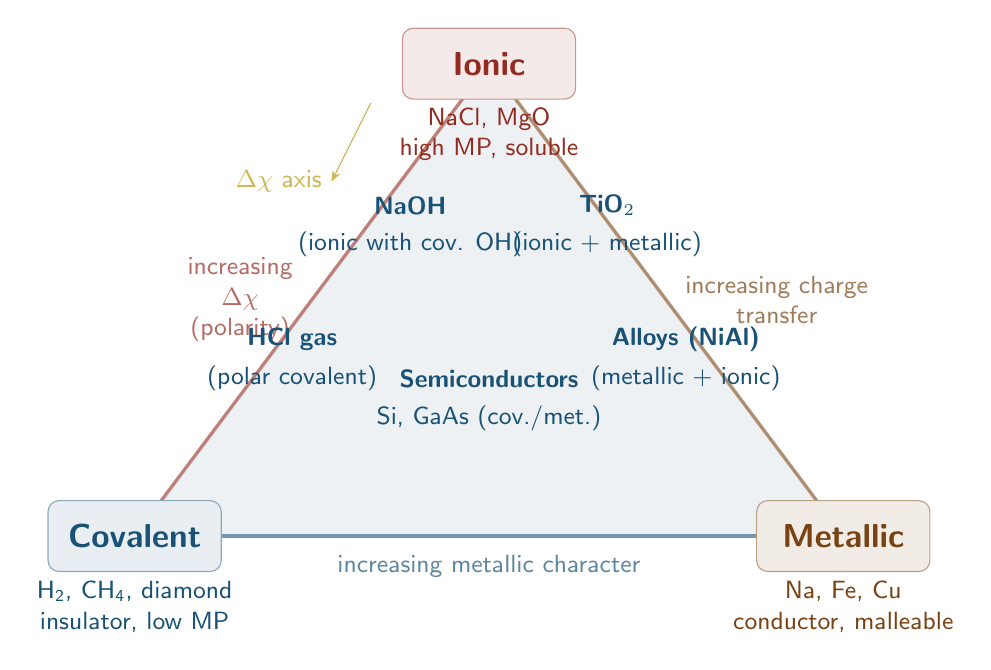
\begin{tikzpicture}[every node/.style={font=\sffamily\small, align=center},
                    scale=1.0]

  % Triangle vertices
  \coordinate (ionic)  at (0, 6.0);
  \coordinate (coval)  at (-4.5, 0);
  \coordinate (metal)  at (4.5, 0);

  % Gradient fills (rough, manual)
  % Fill the triangle with a blend
  \fill[JourneyColor!8] (ionic) -- (coval) -- (metal) -- cycle;

  % Triangle edges
  \draw[very thick, IonicCorner!60] (ionic) -- (coval)
    node[midway, left=3pt, font=\sffamily\small, text=IonicCorner!70]
      {increasing\\$\Delta\chi$\\(polarity)};
  \draw[very thick, CovalCorner!60] (coval) -- (metal)
    node[midway, below=3pt, font=\sffamily\small, text=CovalCorner!70]
      {increasing metallic character};
  \draw[very thick, MetalCorner!60] (metal) -- (ionic)
    node[midway, right=3pt, font=\sffamily\small, text=MetalCorner!70]
      {increasing charge\\transfer};

  % Vertex labels
  \node[font=\sffamily\large\bfseries, text=IonicCorner,
        draw=IonicCorner!50, fill=IonicCorner!10, rounded corners,
        minimum width=2.2cm, minimum height=0.9cm]
    at (ionic) {Ionic};
  \node[font=\sffamily\small, text=IonicCorner]
    at ($(ionic) + (0,-0.9)$) {NaCl, MgO\\high MP, soluble};

  \node[font=\sffamily\large\bfseries, text=CovalCorner,
        draw=CovalCorner!50, fill=CovalCorner!10, rounded corners,
        minimum width=2.2cm, minimum height=0.9cm]
    at (coval) {Covalent};
  \node[font=\sffamily\small, text=CovalCorner]
    at ($(coval) + (0,-0.9)$) {\ce{H2}, \ce{CH4}, diamond\\insulator, low MP};

  \node[font=\sffamily\large\bfseries, text=MetalCorner,
        draw=MetalCorner!50, fill=MetalCorner!10, rounded corners,
        minimum width=2.2cm, minimum height=0.9cm]
    at (metal) {Metallic};
  \node[font=\sffamily\small, text=MetalCorner]
    at ($(metal) + (0,-0.9)$) {Na, Fe, Cu\\conductor, malleable};

  % Interior substance labels
  \node[font=\sffamily\small\bfseries, text=JourneyColor]
    at (-1.0, 4.2) {NaOH};
  \node[font=\sffamily\small, text=JourneyColor]
    at (-1.0, 3.7) {(ionic with cov. OH)};

  \node[font=\sffamily\small\bfseries, text=JourneyColor]
    at (1.5, 4.2) {TiO$_2$};
  \node[font=\sffamily\small, text=JourneyColor]
    at (1.5, 3.7) {(ionic + metallic)};

  \node[font=\sffamily\small\bfseries, text=JourneyColor]
    at (0, 2.0) {Semiconductors};
  \node[font=\sffamily\small, text=JourneyColor]
    at (0, 1.5) {Si, GaAs (cov./met.)};

  \node[font=\sffamily\small\bfseries, text=JourneyColor]
    at (-2.5, 2.5) {HCl gas};
  \node[font=\sffamily\small, text=JourneyColor]
    at (-2.5, 2.0) {(polar covalent)};

  \node[font=\sffamily\small\bfseries, text=JourneyColor]
    at (2.5, 2.5) {Alloys (NiAl)};
  \node[font=\sffamily\small, text=JourneyColor]
    at (2.5, 2.0) {(metallic + ionic)};

  % Electronegativity axis annotation
  \draw[-{Stealth[length=4pt]}, thin, DiscoveryColor!70]
    (-1.5,5.5) -- (-2.0,4.5)
    node[left, font=\sffamily\small, text=DiscoveryColor!70]
      {$\Delta\chi$ axis};

\end{tikzpicture}
\end{center}

\vspace{0.4em}

The position within the triangle is determined by:
\begin{itemize}[nosep, leftmargin=2em]
  \item \textbf{Vertical position}: the electronegativity
        difference $\Delta\chi$ between the two elements.
        High $\Delta\chi$ (metal + nonmetal) $\to$ ionic vertex.
        Low $\Delta\chi$ $\to$ covalent or metallic.
  \item \textbf{Horizontal position}: whether both elements
        are nonmetals (left, covalent) or metals (right, metallic).
\end{itemize}

\subsection{Predicting Properties from Position}

\begin{center}
\small
\begin{tabular}{p{2.8cm}llllll}
\toprule
Substance & Bond type & Conducts? & MP & Soluble (H$_2$O)? & Hard? \\
\midrule
NaCl  & ionic          & molten/aq & high & yes (polar)  & brittle \\
MgO   & ionic          & molten/aq & very high & low  & very hard \\
\ce{CH4}  & cov.\ + LDF & no   & very low & no           & soft (gas) \\
Diamond   & cov.\ network & no & very high & no           & hardest known \\
Graphite  & cov.\ $\sigma$ + deloc.\ $\pi$ & yes (2D) & very high & no & soft (layers slide) \\
Copper    & metallic    & yes  & high & no (reacts)  & malleable \\
SiC       & cov.\ network & no & very high & no           & very hard \\
Ice       & cov.\ + H-bond & no & moderate & yes          & moderate \\
\bottomrule
\end{tabular}
\end{center}

\subsection{The Bonding Continuum in Action: Ketelaar's Triangle}

Ketelaar (1946) formalised the bonding triangle using
electronegativity values.
For a compound AB:
\begin{itemize}[nosep, leftmargin=2em]
  \item \textbf{Average electronegativity} $(\chi_A + \chi_B)/2$:
        determines metallic vs nonmetallic character
        (high average $\to$ nonmetal/covalent side).
  \item \textbf{Electronegativity difference} $|\chi_A - \chi_B|$:
        determines ionic character (high difference $\to$ ionic).
\end{itemize}

\begin{namedconcept}{Ketelaar's Triangle: Quantitative Placement}
\begin{center}
\small
\begin{tabular}{lllll}
\toprule
Compound & $\chi_A$ & $\chi_B$ & Average & Difference \\
\midrule
CsF  & 0.79 & 3.98 & 2.39 & 3.19 (ionic) \\
NaCl & 0.93 & 3.16 & 2.05 & 2.23 (ionic) \\
HCl  & 2.20 & 3.16 & 2.68 & 0.96 (polar cov.) \\
HF   & 2.20 & 3.98 & 3.09 & 1.78 (polar cov. / ionic) \\
CO   & 2.55 & 3.44 & 3.00 & 0.89 (polar cov.) \\
\ce{N2}  & 3.04 & 3.04 & 3.04 & 0.00 (pure cov.) \\
Li   & 0.98 & 0.98 & 0.98 & 0.00 (metallic) \\
NiAl & 1.91 & 1.61 & 1.76 & 0.30 (metallic-ionic) \\
\bottomrule
\end{tabular}
\end{center}
\end{namedconcept}

\begin{problembox}
\begin{enumerate}[label=\textbf{\arabic*.}]
  \item \textbf{Identifying bonding from data.}

    Identify the dominant bonding type in each substance
    from the following physical property data, and place
    each approximately in Ketelaar's triangle:

    \begin{center}
    \small
    \begin{tabular}{lllll}
    \toprule
    Substance & MP ($^\circ$C) & Conducts (solid)? & Conducts (melt)? & Soluble? \\
    \midrule
    A & 2730  & No  & No  & No \\
    B & 801   & No  & Yes & Yes \\
    C & $-115$& No  & No  & Yes (reacts with \ce{H2O}) \\
    D & 1084  & Yes & Yes & No \\
    E & 3550  & No  & No  & No \\
    \bottomrule
    \end{tabular}
    \end{center}
    Candidates: diamond, NaCl, copper, \ce{PCl3}, MgO.

  \item \textbf{Connected prediction.}

    Silicon carbide (SiC) is used in cutting tools and
    high-temperature furnace components.
    \begin{enumerate}[label=(\alph*)]
      \item Using electronegativity values
            (Si: 1.90, C: 2.55) and Ketelaar's triangle,
            classify the Si--C bond.
      \item Both Si and C form $sp^3$ networks.
            Predict the crystal structure of SiC.
      \item SiC has a Young's modulus of $\sim 450$ GPa
            (compare: steel $\sim 200$ GPa, diamond $\sim 1000$ GPa).
            Explain the trend: diamond $>$ SiC $>$ steel in
            stiffness, using the bonding in each material.
      \item SiC is a semiconductor with a band gap of $\sim 3$ eV
            (wide bandgap, vs Si at $1.1$ eV).
            Suggest why a wider band gap makes SiC better for
            high-temperature electronics (hint: thermal excitation).
    \end{enumerate}

  \item \textbf{From formula to properties.}

    For each of the following, predict from the formula alone:
    the melting point range (very high $>1000^\circ$C,
    moderate $200$--$1000^\circ$C, low $<200^\circ$C),
    whether it dissolves in water, and whether it conducts
    electricity as a solid:
    \begin{enumerate}[label=(\alph*)]
      \item \ce{K2O}
      \item \ce{SiO2}
      \item \ce{PCl5}
      \item \ce{Al}
      \item \ce{CaCO3}
      \item \ce{C60} (buckminsterfullerene)
    \end{enumerate}
\end{enumerate}
\end{problembox}

\subsection*{Journey 4 Synthesis}

\begin{synthbox}
Journey~4 has built the complete picture of chemical bonding
from its quantum mechanical foundation to its macroscopic consequences.

\begin{center}
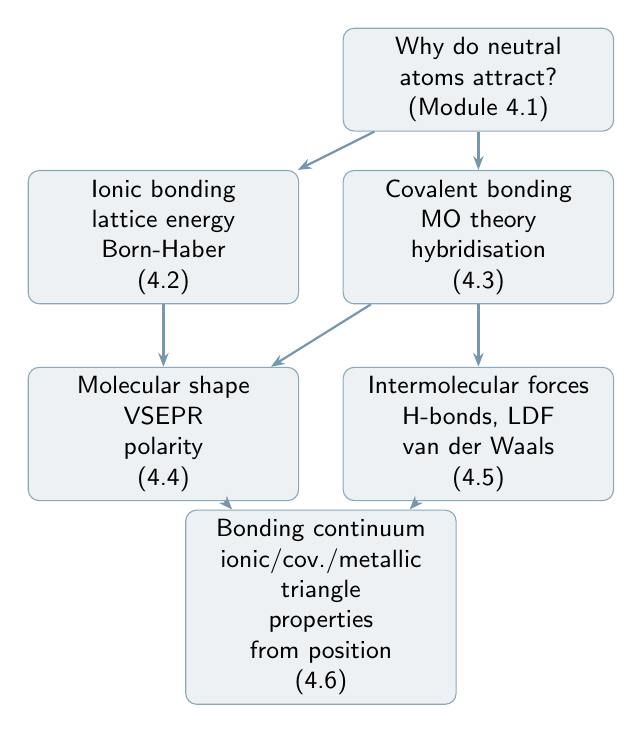
\begin{tikzpicture}[
  every node/.style={font=\sffamily\small, align=center},
  box/.style={draw=JourneyColor!50, fill=JourneyColor!8, rounded corners=4pt,
              minimum width=3.4cm, minimum height=1.0cm, text width=3.2cm},
  arr/.style={-{Stealth[length=5pt]}, thick, JourneyColor!60}
]
  \node[box] (puzzle) at (0,6.5)
    {Why do neutral atoms attract?\\(Module 4.1)};
  \node[box] (ionic)  at (-4,4.5)
    {Ionic bonding\\lattice energy\\Born-Haber\\(4.2)};
  \node[box] (coval)  at (0,4.5)
    {Covalent bonding\\MO theory\\hybridisation\\(4.3)};
  \node[box] (shape)  at (-4,2.0)
    {Molecular shape\\VSEPR\\polarity\\(4.4)};
  \node[box] (imf)    at (0,2.0)
    {Intermolecular forces\\H-bonds, LDF\\van der Waals\\(4.5)};
  \node[box] (synth)  at (-2.0,-0.2)
    {Bonding continuum\\ionic/cov./metallic triangle\\properties from position\\(4.6)};

  \draw[arr] (puzzle) -- (ionic);
  \draw[arr] (puzzle) -- (coval);
  \draw[arr] (ionic)  -- (shape);
  \draw[arr] (coval)  -- (shape);
  \draw[arr] (coval)  -- (imf);
  \draw[arr] (shape)  -- (synth);
  \draw[arr] (imf)    -- (synth);
\end{tikzpicture}
\end{center}

\medskip
\textbf{The six things Journey~4 established:}
\begin{enumerate}[nosep, leftmargin=2em]
  \item Chemical bonds form because quantum mechanics allows
        electrons to lower their kinetic energy by delocalising
        over larger spaces (particle-in-a-box principle).
  \item Ionic bonds are pure electrostatics in a lattice.
        Stability requires lattice energy to exceed ionisation
        energy. Both scale as $z_+z_-/r_0$.
  \item Covalent bonds arise from constructive interference
        of wave functions. Bond order from MO theory
        quantitatively predicts bond length and strength.
        MO theory explains \ce{O2} paramagnetism; Lewis theory does not.
  \item Molecular geometry follows from electron pair repulsion
        (VSEPR). Shape determines polarity; polarity determines
        most physical properties.
  \item Intermolecular forces are 10--100$\times$ weaker than
        bonds, yet determine boiling points, solubility, and
        all of structural biology.
        H-bonds are the pivot of living chemistry.
  \item Ionic, covalent, and metallic are not distinct categories
        but the vertices of a continuum triangle.
        Every substance sits somewhere inside.
\end{enumerate}
\end{synthbox}

\subsection*{Deep Problems}

\begin{deepbox}
\begin{enumerate}[label=\textbf{D\arabic*.}]

  \item \textbf{From bond energies to thermochemistry to biology.}

    Glucose (\ce{C6H12O6}) is metabolised in cells:
    \[
      \ce{C6H12O6(aq) + 6O2(g) -> 6CO2(g) + 6H2O(l)}
    \]
    $\Delta H = -2803$ kJ/mol.

    \begin{enumerate}[label=(\alph*)]
      \item Using bond energies, estimate $\Delta H$ for
            the gas-phase reaction (treat glucose as
            having 5 C--C, 7 C--H, 5 C--O, 1 C=O bonds
            and appropriate O--H bonds).
            Compare to the actual value.
      \item The cellular efficiency of extracting this energy
            as ATP is $\sim 40\%$.
            How many kJ per mol ATP are stored?
            (Hint: 38 ATP per glucose, each requiring
            $\sim 30.5$ kJ to form.)
      \item The human body needs $\sim 8000$ kJ/day.
            How many moles of glucose must be metabolised?
      \item ATP hydrolysis (\ce{ATP + H2O -> ADP + Pi},
            $\Delta G = -30.5$ kJ/mol) drives muscle
            contraction. The phosphate bond is sometimes
            called a ``high-energy bond.''
            Using what you know about bond energies,
            explain why the phosphate bond itself is not
            actually a particularly strong bond --- the
            energy comes from elsewhere.
    \end{enumerate}

  \item \textbf{Graphene: the bonding that defied expectation.}

    Graphene is a single layer of carbon atoms in a hexagonal
    lattice. Each carbon is $sp^2$ hybridised with one
    unhybridised $p_z$ orbital perpendicular to the plane.

    \begin{enumerate}[label=(\alph*)]
      \item Each C has three $\sigma$ bonds ($sp^2$--$sp^2$)
            and participates in a delocalised $\pi$ system.
            The C--C bond length in graphene is 142 pm,
            between single (154 pm) and double (134 pm).
            Explain using bond order and delocalisation.
      \item The delocalised $\pi$ electrons can move freely
            across the entire graphene sheet.
            Explain why graphene conducts electricity
            despite being pure carbon covalent solid
            (a ``semiconductor'' with zero band gap).
      \item Diamond (all C--C, $sp^3$, no delocalisation)
            is an electrical insulator. Graphite and graphene
            conduct. The only difference is hybridisation.
            \textbf{What does this tell us about the connection
            between molecular orbital theory and the
            electrical properties of materials?}
      \item Graphene has exceptional mechanical strength
            (Young's modulus $\sim 1000$ GPa).
            Compare this to diamond ($\sim 1000$ GPa)
            and explain why two such different structural forms
            of carbon have similar stiffness.
    \end{enumerate}

\end{enumerate}
\end{deepbox}

\subsection*{Reflection}

\begin{reflectionbox}
\begin{enumerate}[label=\textbf{R\arabic*.}]
  \item Journey~4 has shown that all bonding --- ionic,
    covalent, metallic, intermolecular --- traces to the
    same origin: the quantum mechanical behaviour of electrons
    in the field of positive nuclei.
    \textbf{Is there a sense in which all of chemistry is
    just one phenomenon viewed from different angles?}
    Or are the bond types genuinely different in kind?

  \item The H-bond in DNA ($\sim 20$ kJ/mol) is about 8 times
    larger than thermal energy at body temperature.
    Yet DNA can be opened by polymerases at room temperature.
    \textbf{What does this tell us about the relationship
    between bond energy and reaction kinetics?}
    Why does a thermodynamically ``stable'' bond not imply
    a ``slow'' reaction?

  \item We built up from the Schr\"{o}dinger equation
    (Journey~2) to periodic trends (Journey~3)
    to bond types (Journey~4).
    At each step, emergent properties arose that weren't
    visible at the level below.
    \textbf{Is chemistry ``just'' applied quantum mechanics,
    or does each level of organisation have its own
    irreducible concepts?}
    What is lost if we always ``explain'' chemistry by reducing
    it to physics?
\end{enumerate}
\end{reflectionbox}

\vspace{1.5em}
\begin{center}
\begin{tcolorbox}[enhanced,
  colback=JourneyColor!12, colframe=JourneyColor,
  width=0.9\textwidth, arc=4pt]
\centering\sffamily
\textbf{\large Journey 4 Complete: The Bond --- Why Atoms Stick Together}\\[8pt]
\small
\begin{tabular}{ll}
Module 4.1 & The bonding puzzle: neutral atoms attract via QM delocalisation \\
Module 4.2 & Ionic bonding: Madelung lattice energy, Born-Haber cycle \\
Module 4.3 & Covalent bonding: MO theory, $\sigma$/$\pi$ bonds, O$_2$ paramagnetism \\
Module 4.4 & Molecular shape: VSEPR, polarity, geometry from pairs \\
Module 4.5 & Intermolecular forces: LDF, H-bonds, van der Waals \\
Module 4.6 & Synthesis: the bonding continuum triangle \\
\end{tabular}\\[8pt]
\textit{Continue to Journey~5: Reactions --- The Grammar of Chemistry.}
\end{tcolorbox}
\end{center}

\end{document}